\documentclass[11pt,a4paper]{article}
\usepackage[utf8]{inputenc}
\usepackage[spanish]{babel}
\usepackage{amsmath, amssymb}
\usepackage{graphicx}
\usepackage[margin=2.5cm]{geometry}
\usepackage{fancyhdr}
\usepackage{tcolorbox}
\usepackage{enumitem}

\definecolor{UCBblue}{RGB}{0, 51, 153}
\definecolor{UCBgray}{RGB}{100, 100, 100}
\definecolor{UCBred}{RGB}{153, 0, 0}

\pagestyle{fancy}
\fancyhf{}
\fancyhead[L]{\textcolor{UCBblue}{\textbf{Ingeniería Mecatrónica - UCB Tarija}}}
\fancyhead[R]{\textcolor{UCBgray}{Taller de Nivelación / Intro. a la Mecatrónica}}
\fancyfoot[C]{\thepage}
\renewcommand{\headrulewidth}{0.4pt}
\renewcommand{\headrule}{\hbox to\headwidth{\color{UCBblue}\leaders\hrule height \headrulewidth\hfill}}

\begin{document}

\begin{center}
    {\Large \textbf{\textcolor{UCBblue}{Guía de Modelado Analítico: Sistematización de Redes de Potencia}}}\\
    \vspace{0.3cm}
    {\large \textbf{Fase CDIO: Concebir (Fundamentos y Aplicación de LVK)}}\\
    \vspace{0.5cm}
    \textbf{Estudiante:} \rule{8cm}{0.4pt} \quad \textbf{Fecha:} \rule{3cm}{0.4pt}
\end{center}

\vspace{0.3cm}

\section*{1. Glosario Físico-Matemático Fundamental}
Para evitar que el álgebra lineal se reduzca a la manipulación abstracta de números, establecemos las siguientes definiciones rectoras para el modelado de hardware:

\begin{itemize}
    \item \textbf{Ley de Voltajes de Kirchhoff (LVK):} Es el principio de conservación de la energía en un circuito cerrado. La energía suministrada por las fuentes activas ($\mathbf{V}$) es exactamente igual a la energía disipada térmicamente por los elementos pasivos ($\mathbf{R}$).
    \item \textbf{La Matriz ($\mathbf{R}$) y el Vector ($\mathbf{I}$):} $\mathbf{R}$ no es una tabla de números, es el \textit{mapa topológico} que cuantifica la oposición estructural de la red. $\mathbf{I}$ es el \textit{vector de estado}, nuestra incógnita principal que dictará el flujo real de electrones hacia los actuadores.
\end{itemize}

\section*{2. Formulación Algebraica de la LVK (El Paso a Paso)}
Antes de ensamblar la matriz $\mathbf{R}$, debemos plantear la ecuación algebraica de conservación de energía ($\sum V = 0$) para cada malla. Siga este rigor procedimental:

\begin{tcolorbox}[colback=white,colframe=UCBblue,title=\textbf{Algoritmo Analítico de Lazo Cerrado}]
\textbf{Paso 1: Asignación de Variables} \\
Dibuje una trayectoria de corriente en sentido horario ($\circlearrowright$) en cada malla independiente ($I_1, I_2, I_3$).

\vspace{0.2cm}
\textbf{Paso 2: Sumatoria de Caídas de Tensión (Lado Izquierdo)} \\
Recorra la malla siguiendo la flecha de su corriente. Al pasar por una resistencia $R$, se produce una caída de tensión (Ley de Ohm: $V = R \cdot I$).
\begin{itemize}
    \item Si la resistencia es \textbf{propia} (solo pasa su corriente $I_1$), anote: $+ R \cdot I_1$.
    \item Si la resistencia es \textbf{compartida} con otra malla (ej. $I_2$), anote el efecto neto: $+ R \cdot (I_1 - I_2)$.
\end{itemize}

\vspace{0.2cm}
\textbf{Paso 3: Balance con Fuentes Activas (Lado Derecho)} \\
Iguale la sumatoria anterior a las fuentes de voltaje de la malla. Observe por qué terminal ingresa su trayectoria de corriente a la batería:
\begin{itemize}
    \item Si ingresa por el terminal \textbf{negativo} (trazo corto), anote el valor de la fuente como \textbf{positivo}.
    \item Si ingresa por el terminal \textbf{positivo} (trazo largo), anote el valor como \textbf{negativo}.
\end{itemize}
\end{tcolorbox}

\section*{3. Sistematización Matricial}
Una vez formuladas las ecuaciones algebraicas, el reordenamiento de los términos genera la estructura canónica $\mathbf{R}\mathbf{I} = \mathbf{V}$:
\begin{itemize}
    \item \textbf{Diagonal Principal ($R_{kk}$):} Suma de todas las resistencias del lazo $k$ (Siempre positivo).
    \item \textbf{Extradiagonales ($R_{kj}$):} Resistencia compartida entre el lazo $k$ y $j$ (Precedida por un signo negativo).
\end{itemize}

\section*{4. Escalonamiento del Determinante}
\begin{tcolorbox}[colback=blue!5!white,colframe=UCBblue,title=\textbf{A. Concepto Base (Matriz $2\times2$)}]
$$ \mathbf{R} = \begin{bmatrix} a & b \\ c & d \end{bmatrix} \implies \det(\mathbf{R}) = (a \cdot d) - (b \cdot c) $$
\end{tcolorbox}

\begin{tcolorbox}[colback=blue!5!white,colframe=UCBblue,title=\textbf{B. Expansión Visual a $3\times3$ (Regla de Sarrus)}]
\textbf{Limitación Crítica:} Este patrón visual \textit{solo es válido para matrices de $3\times3$}. Carece de validez matemática para dimensiones $4\times4$ o superiores.
\end{tcolorbox}

\newpage

\section*{5. Desarrollo Analítico: Misión de Ingeniería}

\begin{figure}[h!]
    \centering
    \framebox[14cm][c]{\rule{0pt}{6cm} 
    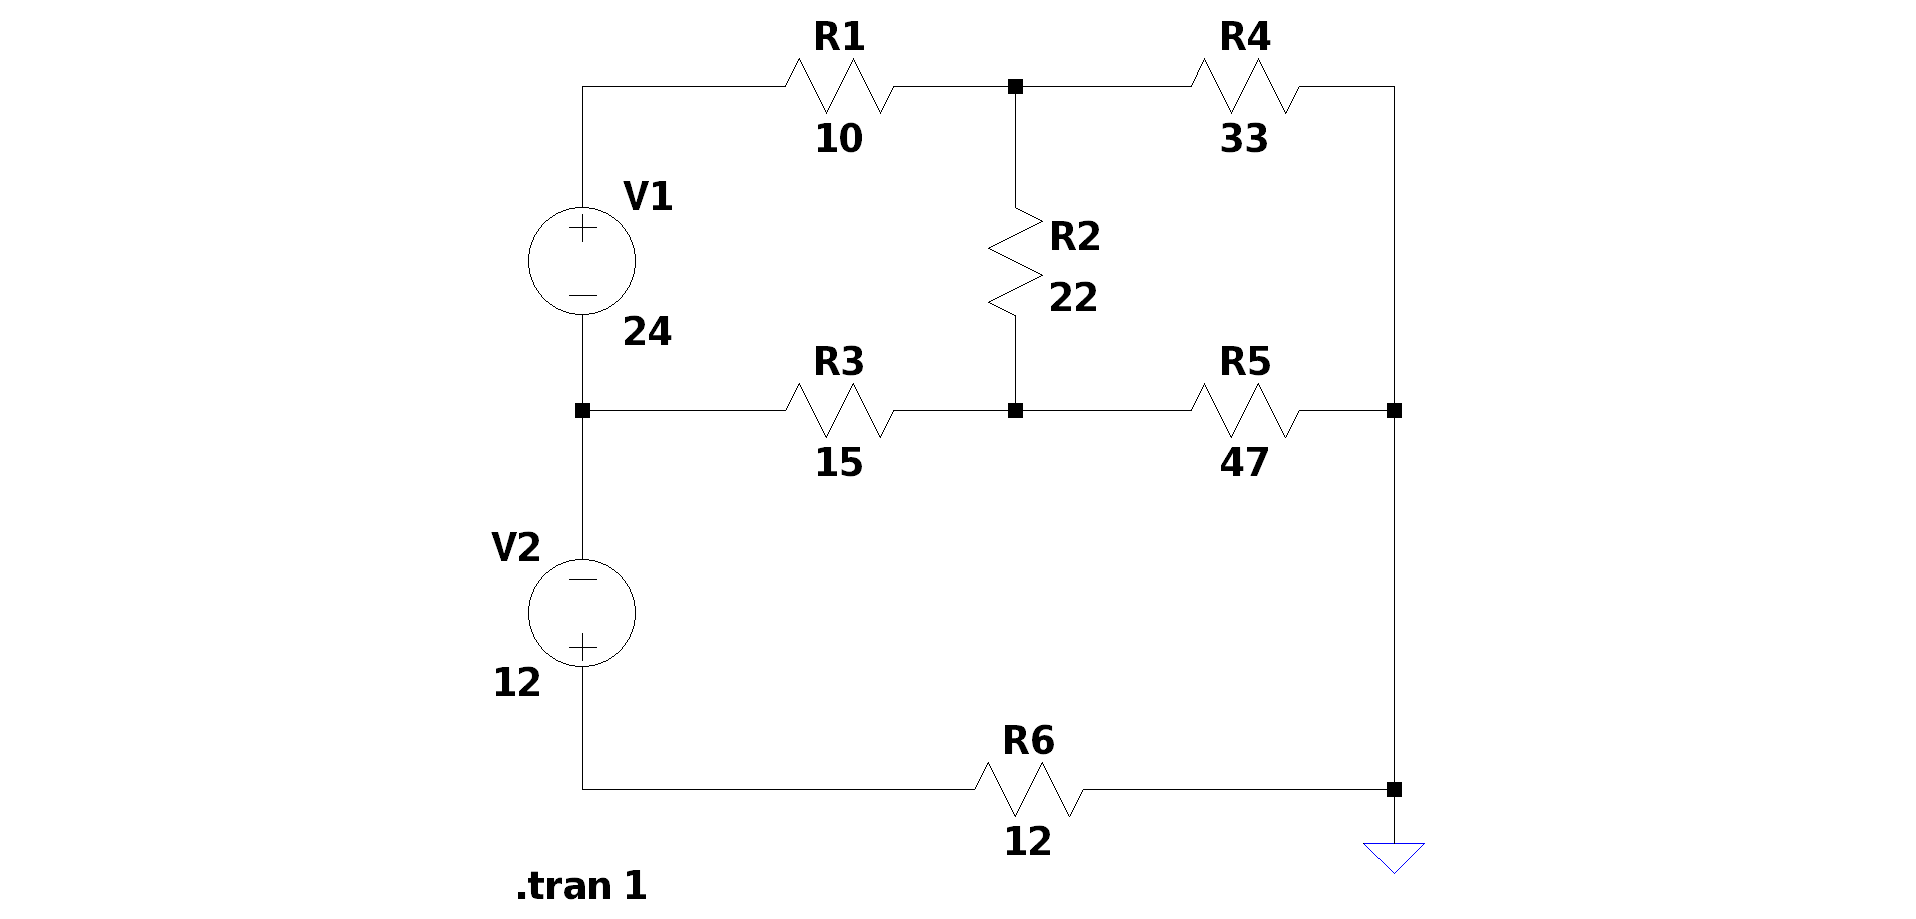
\includegraphics{schematic.png}
    }
    \caption{Topología coplanar de la red de distribución de potencia mecatrónica.}
\end{figure}

Considere: $R_1=10\Omega, R_2=22\Omega, R_3=15\Omega, R_4=33\Omega, R_5=47\Omega, R_6=12\Omega$ y $V_{s1}=24V, V_{s2}=0V, V_{s3}=-12V$.

\textbf{A.} Utilice el "Algoritmo Analítico de Lazo Cerrado" (Paso a Paso) para deducir la ecuación de la \textbf{Malla 1} \textit{antes} de ensamblar la matriz:
\begin{tcolorbox}[colback=white,colframe=UCBgray,height=2.5cm,valign=top]
\textit{Ecuación algebraica Malla 1 ($\sum V_{\text{caídas}} = \sum V_{\text{fuentes}}$):}
\end{tcolorbox}

\textbf{B.} Ensamble la Matriz $\mathbf{R}$ garantizando la simetría y positividad diagonal:
\vspace{0.1cm}
$$
\begin{bmatrix}
 \dots \dots \dots & \dots \dots & \dots \dots \\
 \dots \dots \dots & \dots \dots \dots & \dots \dots \\
 \dots \dots \dots & \dots \dots \dots & \dots \dots \dots
\end{bmatrix}
\begin{bmatrix}
 I_1 \\
 I_2 \\
 I_3
\end{bmatrix}
=
\begin{bmatrix}
 \dots \dots \\
 \dots \dots \\
 \dots \dots
\end{bmatrix}
$$
\vspace{0.1cm}

\textbf{C.} Evalúe el determinante principal de la matriz mediante la \textbf{Regla de Sarrus}.

\begin{tcolorbox}[colback=white,colframe=UCBgray,height=3cm,valign=top]
\textit{Desarrollo analítico de Sarrus:}
\end{tcolorbox}

\end{document}
